% This is samplepaper.tex, a sample chapter demonstrating the
% LLNCS macro package for Springer Computer Science proceedings;
% Version 2.20 of 2017/10/04
%
\documentclass[runningheads]{llncs}
%
\usepackage{graphicx}
\usepackage{multirow} 
\usepackage{fancyvrb}
\usepackage[misc,geometry]{ifsym} 
\usepackage{subcaption}
\usepackage{caption}
% Used for displaying a sample figure. If possible, figure files should
% be included in EPS format.
%
% If you use the hyperref package, please uncomment the following line
% to display URLs in blue roman font according to Springer's eBook style:
% \renewcommand\UrlFont{\color{blue}\rmfamily}

\begin{document}
%
\title{Formal Grammars and Residual Neural Networks for RNA Secondary Structure Prediction\thanks{Supported by the Russian Science Foundation grant 18-11-00100}}
%
%\titlerunning{Abbreviated paper title}
% If the paper title is too long for the running head, you can set
% an abbreviated paper title here
%
\author{Polina Lunina\inst{1,2}\orcidID{0000-0002-7172-2647} \Letter \and
Semyon Grigorev\inst{1,2}\orcidID{0000-0002-7966-0698} \and
Vadim Abzalov\inst{1,2}\orcidID{0000-0002-0805-0315}}
%
\authorrunning{Polina Lunina, Semyon Grigorev, Vadim Abzalov}
% First names are abbreviated in the running head.
% If there are more than two authors, 'et al.' is used.
%
\institute{Saint Petersburg State University, 7/9 Universitetskaya nab., St. Petersburg, 199034, Russia \and
JetBrains Research, Primorskiy prospekt 68-70, Building 1, St. Petersburg 197374, Russia\\
\email{lunina\_polina@mail.ru \Letter, semyon.grigorev@jetbrains.com, vadim.i.abzalov@gmail.com}\\
}
%
\maketitle             % typeset the header of the contribution
%
\begin{abstract}
RNA secondary structure prediction task is known to be quite critical in computational genomics, therefore, different tools and algorithms are still competing in this field. In this work, we propose to combine formal grammars and neural networks to solve this problem. Our approach utilizes the idea that RNA secondary structure can be viewed as recursive composition of various stems. We describe the most probable types of stems by simple context-free grammar, so that parsing matrix for some sequence would represent all the theoretically possible stems. Then we process these matrices with residual neural networks in order to generate a valid secondary structure. This approach allows to process pseudoknotted structures, non-canonical base pairs and multiple contacts due to flexible nature of neural network training process.

\keywords{CNN \and ResNet \and Machine Learning \and Secondary Structure \and Genomic Sequences \and Formal Grammars \and Parsing.}
\end{abstract}
%
%
%
\section{Introduction}
Improvement in RNA secondary structure prediction accuracy is one of the key focuses in computational genomics due to its crucial role in functional analysis of RNA molecules. All the diversity of existing secondary structure prediction techniques can be divided into comparative methods that analyse several homologous sequences employing evolutionary approaches~\cite{hofacker1999automatic,tahi2002automatic} and single sequence methods that process one sequence at a time according to some folding constraints, e.g. thermodynamic~\cite{hamada2009prediction} or statistic~\cite{eddy1994rna,do2006contrafold} rules. One of the challenging parts is pseudoknotted structures processing, because pseudoknots are known to be widely represented in biological data, including functionally important RNA regions, nevertheless, building a model that handles them has always been a non-trivial task.

Among other ways, formal grammars can be applied for RNA secondary structure description and some of the algorithms utilize this technique for secondary structure prediction~\cite{knudsen2003pfold,nebel2011evaluation}. Due to the probabilistic nature of secondary structure formation laws complicated stochastic (probabilistic) grammars are generally used and the classical way here is to create a grammar that models the whole structure. This approach is known to be quite successful, but it also should be mentioned that building such grammar requires a lot of theoretical and practical difficulties. Therefore, we propose a different way --- to encode only stems of secondary structure by simple context-free grammar and leave further processing and probability estimation to machine learning methods that are known to be quite successful in biological data processing~\cite{higashi2009bacteria,sherman2017humidor}. 

So, in this work, we introduce a new approach for RNA secondary structure prediction which employs the combination of ordinary formal grammars and artificial neural networks. The main ideas were outlined in~\cite{grigorevcomposition,lunina2019secondary} and this research is conducted to further development of this approach in the context of secondary structure prediction problem. Secondary structure can be formally described as a compositions of stems having different lengths and loop sizes~\cite{MQbioinformatics19}, so, we propose to use a simple context-free (not probabilistic) grammar to encode the most common types of stems and search for such stems in the input sequences by matrix-based parsing algorithm. Thereby, the parsing matrix for some sequence will contain the information about whether each subsequence of this sequence can fold to stem or not. This matrix is not yet a representation of a valid secondary structure, because it cannot contain all these stems at once and, besides, there can be more complex elements that are not expressible in terms of our grammar (such as pseudoknots and non-canonical base pairs). Therefore, we propose to process such matrices by neural networks that should filter extra stems and add some missing elements in order to generate a maximal approximation of this sequence secondary structure. So, on the one hand, using neural networks allows to skip full formalization of RNA secondary structure and on the other hand, the grammar provides some sort of basis for neural network training.

\section{Proposed Approach Overview}
In this section we focus on the theoretical aspects of the proposed approach that underlie all the experimental research presented in the next section. Firstly, we use formal grammars for secondary structure features description and secondly, we apply neural networks for these features processing and solving secondary structure prediction task.

\subsubsection{Formal Grammars}
As it was mentioned before, our approach employs formal grammar not for modeling the whole secondary structure, but for encoding its simple constructional elements --- stems.

In figure~\ref{gram} grammar $G_0$ that we use in this work as well as in the previous ones is presented. This grammar describes the recursive compositions of stems having height at least 3 (lines \textbf{7-12}) and loop size from 1 up to 20 (line \textbf{3}). Note that these constants are not mandatory and might be defined experimentally for each task. Also, $G_0$ allows only conventional base pairs (line \textbf{5}) and does not express pseudoknots, because adding the rules for both of these features complicates the grammar unacceptably in the context of performance, therefore, we expect the neural network to handle them instead. Also, we consider only stems of height three or more, because including shorter stems would overload the parsing matrix with too much extra information. So, by this rules, a sequence folds to stem $\iff$ it is derivable from start nonterminal $s1$ of $G_0$ (line \textbf{1}).

\begin{figure}[ht]
\begin{Verbatim}[numbers=left,xleftmargin=5mm]
start: stem3<s0>
s0: loop | loop stem3<s0> s0
loop: nucl*[1..20]
nucl: A | U | C | G
stem1<s>: A s U | G s C | U s A | C s G
stem2<s>: stem1<stem1<s>>
stem3<s>: 
      stem1<stem2<s>>
    | A stem3<s> U
    | U stem3<s> A
    | C stem3<s> G
    | G stem3<s> C
\end{Verbatim}
\caption{Context-free grammar $G_0$ for RNA secondary structure stems description}
\label{gram}
\end{figure}

Having a grammar, we want to find all the subsequences of some given sequence that may fold to stems and this is to be done by means of parsing. In all the experiments we use parsing algorithm~\cite{Azimov:2018:CPQ:3210259.3210264} that is based on matrix operations and demonstrates high performance in practice due to the effective use of GPGPU. 

Formally, the result of a matrix-based parsing algorithm for an input string $w$ is an upper-triangular boolean matrix $M_P$, where $M_P [i,j] = 1$ $\iff$ the substring $w[i,j]$ is derivable from grammar start nonterminal. From the practical point of view, this means that parsing matrix contains one in a cell $\iff$ a correspondent substring folds to stem according to the rules of a given grammar, so each stem results in a diagonal chain of ones in the matrix, because if sequence $w_1...w_n$ is a stem than it is clear that $w_2...w_{n - 1}$ is a stem, $w_3...w_{n - 2}$ is a stem and so on while the stem height is at least 3.

In figure~\ref{pars_res} we provide the parsing result for a short RNA sequence and show how parsing matrix maps with secondary structure stems. Each one cell describes the stem of height at least 3, so, this sequence contains two subsequences that may fold to stems of the first nesting level. These stems expected hydrogen bonds along with corresponding matrix cells are painted in two different colors. All nucleotide bonds forming a stem of height three or more are represented by solid lines, moreover, it is obvious that each stem of height three encapsulates stems of heights two and one which are highlighted by dotted lines.

Note that these stems interfere with each other, thereby, secondary structure cannot contain both of them at the same time. So, the parsing matrix for a sequence describes all the theoretically possible folds there, but at the current step we cannot know which one of them would be presented in the real secondary structure. Moreover, $G_0$ has certain limitations, such as stem height, loop size and possible base pairs, so, some of the required stems may be missing in the parsing matrix. While creating a grammar we were guided by two competing ideas: to cover as many types of stems as possible and to stay with adequate amount of extra information in parsing matrix along with acceptable time costs for parsing.

\begin{figure}
\centering
\valign{#\cr
  \hbox{%
    \begin{subfigure}[b]{.6\textwidth}
    \centering
    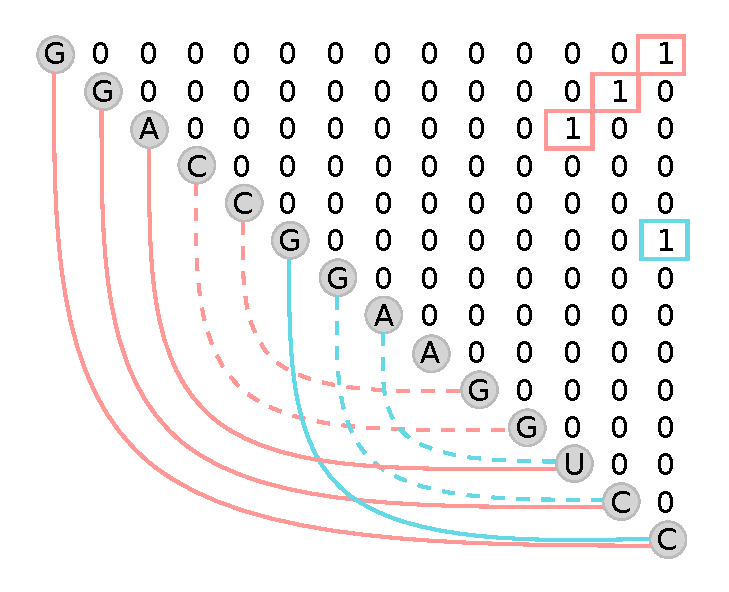
\includegraphics[width=\textwidth]{pics/matrix.pdf}
    \caption{Parsing matrix}
    \label{mtrx}
    \end{subfigure}%
  }\cr
  \noalign{\hfill}
  \hbox{%
    \begin{subfigure}{.4\textwidth}
    \centering
    \vspace{2mm}
    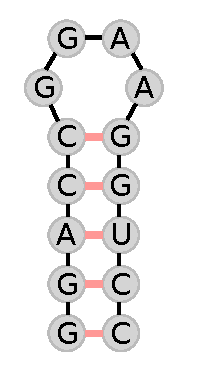
\includegraphics[width=.3\textwidth]{pics/stem1.pdf}
    \caption{First stem}
    \label{stem1}
    \end{subfigure}%
  }\vfill
  \hbox{%
    \begin{subfigure}{.4\textwidth}
    \centering
     \vspace{-2mm}
    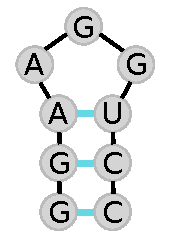
\includegraphics[width=.3\textwidth]{pics/stem2.pdf}
    \caption{Second stem}
    \label{stem2}
    \end{subfigure}%
  }\cr
}
\caption{Stems extracted from RNA sequence}
\label{pars_res}
\end{figure}

Let us consider pseudoknotted structures processing in the context of the proposed approach. Even though it is clear that pseudoknot is not explicitly expressed in $G_0$, it consists of two stem-loop structures having half of one stem located between two halves of another, so, each of these stems separately can be derived by the rules of $G_0$. Therefore, pseudoknots will be reflected in the parsing matrix and handling them becomes an additional task for neural network. In figure~\ref{pk} an example of simple pseudoknot along with corresponding parsing result is provided. Two stems of this pseudoknot are highlighted with two different colors and it can be seen that all the related nucleotide bonds are presented in the parsing matrix, although at this point it is not determined whether sequence contains a pseudoknot or it just has two possible folds in terms of grammar.

\begin{figure}[h]
\centering
\begin{subfigure}{.3\textwidth}
  \centering
  \hbox{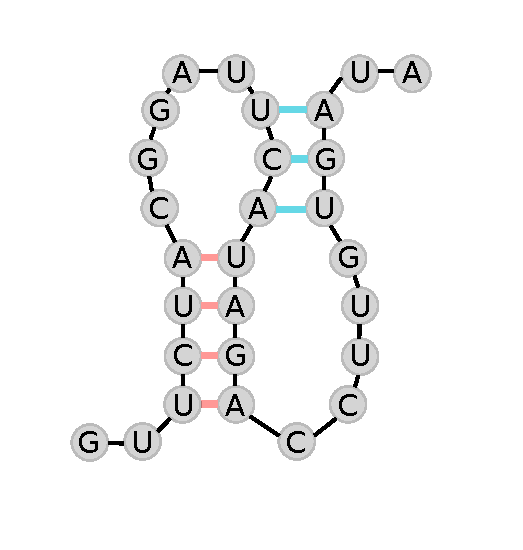
\includegraphics[width=.9\linewidth]{pics/pk.pdf}}
  \caption{Pseudonkot}
  \label{pk_a}
\end{subfigure}%
\begin{subfigure}{.7\textwidth}
  \centering
  \hbox{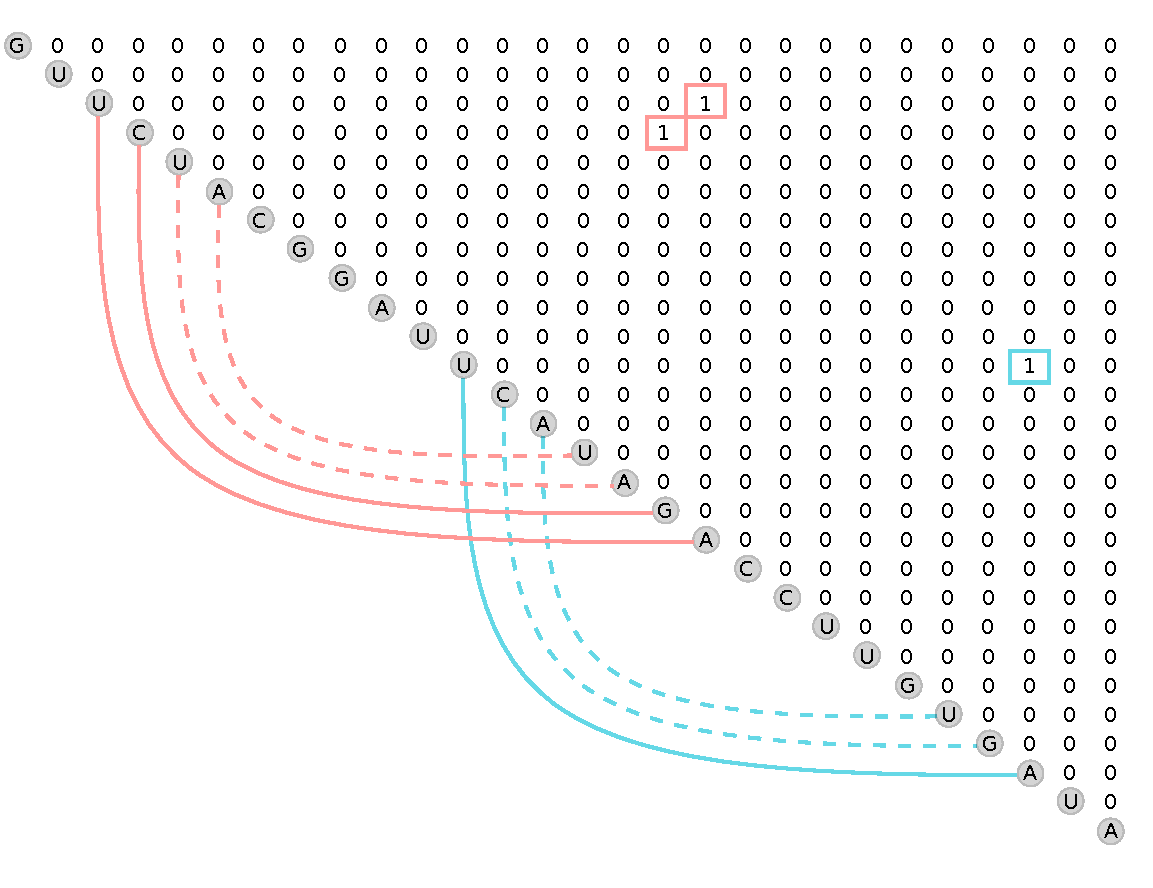
\includegraphics[width=.9\linewidth]{pics/matrix_pk.pdf}}
  \caption{Parsing matrix}
  \label{pk_b}
\end{subfigure}
\caption{Pseudoknots processing in terms of $G_0$}
\label{pk}
\end{figure}

\subsubsection{Neural Networks}
The final step of the proposed solution is to process parsing matrices by a neural network in order to achieve a maximal similarity with the expected sequence secondary structure. Therefore, we need to specify data preparing pipeline and to develop an optimal architecture for a problem at hand. 

\subsubsection{Data}
The input data for neural network (parsing matrices) was described in the previous section and now let us define the reference data source and format. There are specialized biological databases containing RNA chains of various organisms along with their secondary structures obtained by reliable methods and such data is known to be the best for algorithms training and validation. These databases may store data in  different formats (dot-bracket, connectivity table and others), so, we need to choose convenient for our experiments and compatible with others format.

One of the ways of RNA secondary structure formal representation is so-called contact map, which for an input string $w$ is a boolean matrix $M_C$, where $M_C [i,j] = 1$ $\iff$ nucleotides in positions $i$ and $j$ form a hydrogen bond (or, to put it simply, a contact) in secondary structure. Consider the discussed earlier parsing matrix for the same sequence $w$ that has 1 in the cell $[i, j]$ $\iff$ subsequence $w[i, j]$ folds to a stem. It is clear that the first and the last nucleotides of every stem form a contact, therefore, we can easily transfer between parsing matrix and contact map definitions and view the parsing matrix as a sort of a contact map, so, this format is acceptable for our experiments. Note that if parser finds a stem of height three than we will see only one cell with $1$ in matrix, but such stem always wraps a stem of height two which wraps a stem of height one, so, we are always missing two contacts, therefore, after parsing we should set $M_P[i - 1, j + 1] := 1$ , $M_P[i - 2, j + 2] := 1$ if $M_P[i][j] = 1$, $i = 0..size(M_p), j = i + 1..size(M_p)$ for complete equality of these two structures.

So, neural network should take parsing matrices as inputs and contact maps as desired outputs for the same set of RNA sequences. For convenience, we transform both matrices to black-and-white images by replacing zero cells with black pixels and one cells with white pixels. Also, we code RNA sequence at the input image main diagonal by four types of gray pixels corresponding to the four possible nucleotides in case the chain itself contains any important information about secondary structure formation patterns.

In figure~\ref{struc} we provide two-dimensional secondary structure visualization for RNA sequence along with neural network input and reference images that were made from parsing and contact matrices respectively. Contacts belonging to the three stems presented in this sequence are highlighted with three different colors in all pictures (so, input and reference images are actually grayscale, colored pixels are only for clarification). It can be seen that not all of the stems found by parser are presented in the real secondary structure. Moreover, the parsing result is missing several contacts due to the fact that they were formed by non-canonical nucleotide pairs $A-G$ that are not expressed by grammar $G_0$.

\captionsetup[subfigure]{justification=centering}
\begin{figure}[h]
\centering
\begin{subfigure}{.33\textwidth}
  \centering
  \hbox{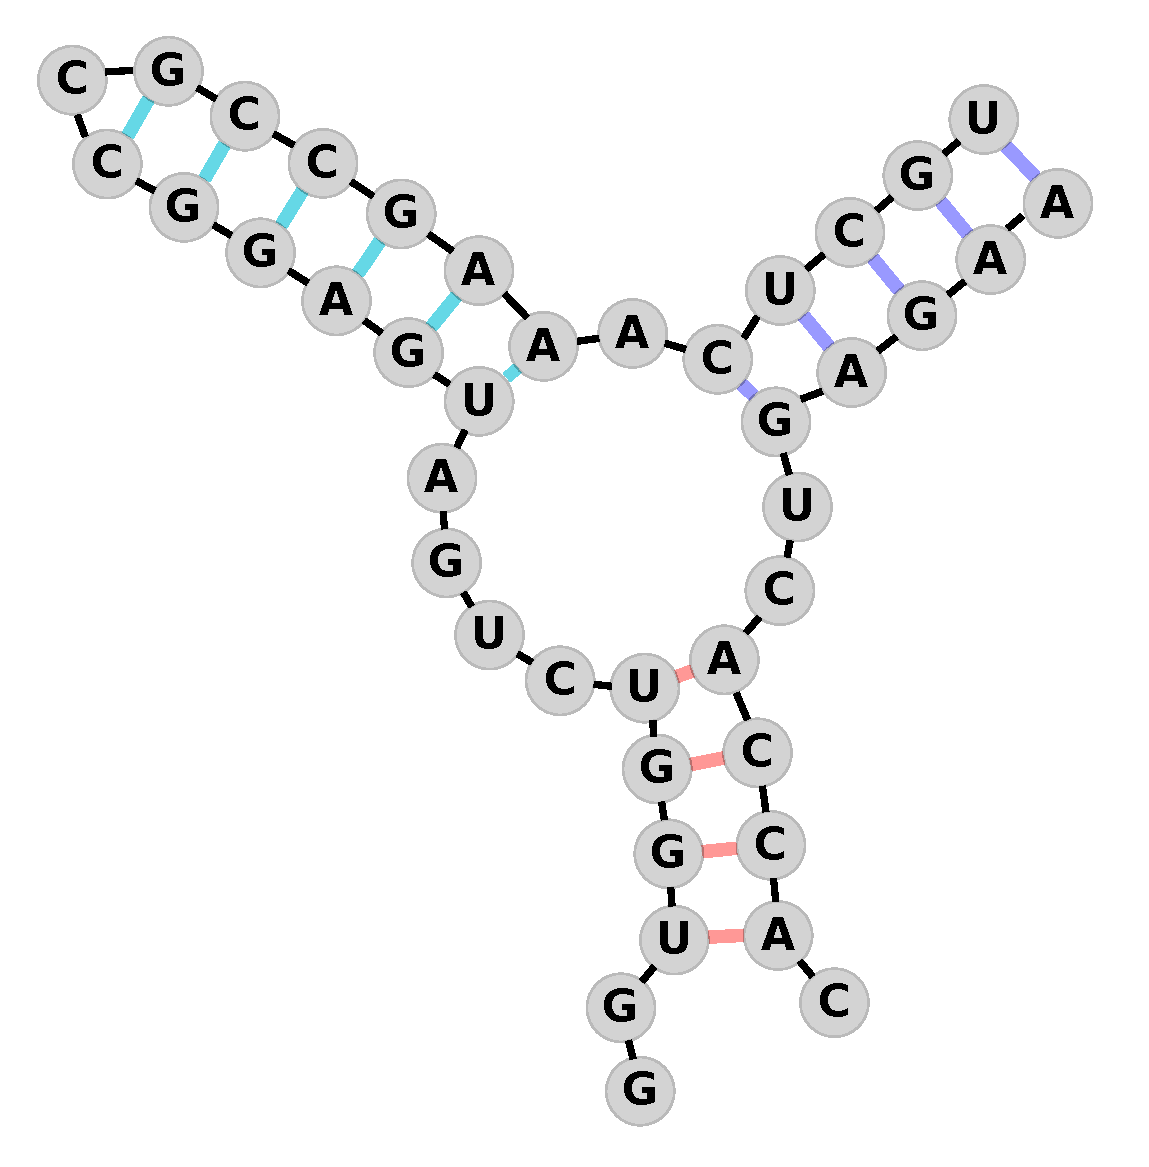
\includegraphics[width=\linewidth]{pics/struct.pdf}}
  \caption{Secondary structure visualization}
  \label{struc_a}
\end{subfigure}%
\begin{subfigure}{.33\textwidth}
  \centering
  \hbox{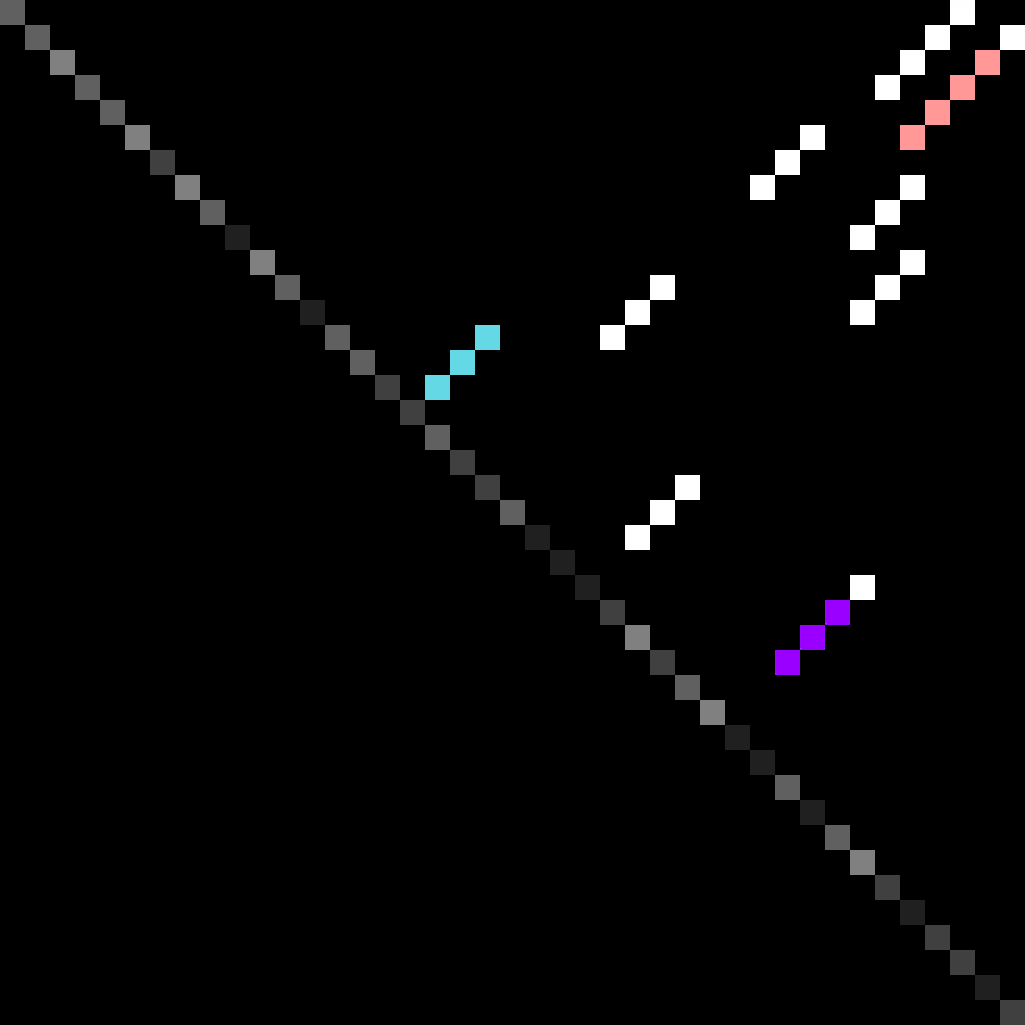
\includegraphics[width=\linewidth]{pics/in.png}}
  \caption{Input image \\ for neural network}
  \label{struc_b}
\end{subfigure}
\begin{subfigure}{.33\textwidth}
  \centering
  \hbox{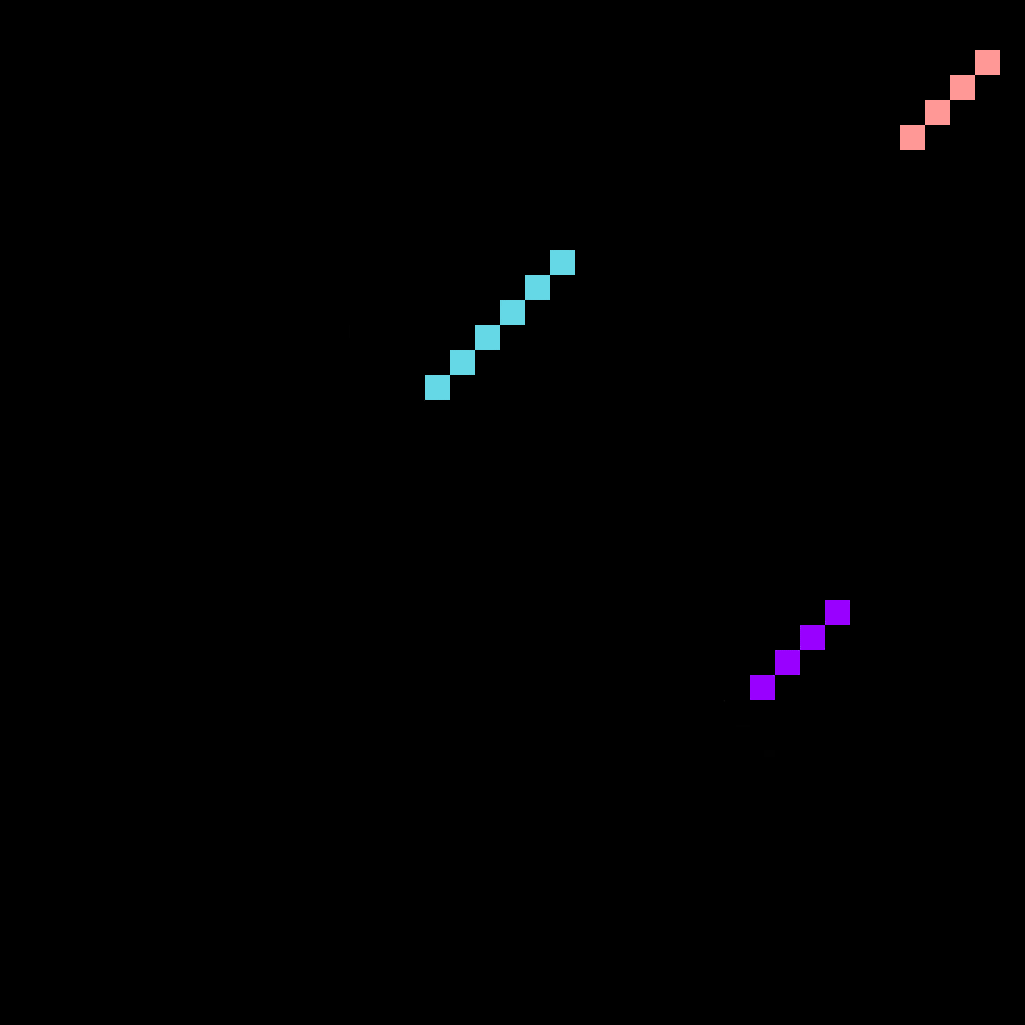
\includegraphics[width=\linewidth]{pics/out.png}}
  \caption{Reference image \\ for neural network}
  \label{struc_c}
\end{subfigure}
\caption{The correspondence between secondary structure stems and pixels in input and reference images}
\label{struc}
\end{figure}

\subsubsection{Parallel ResNet}
One of the popular architectures for complicated image processing tasks is residual neural network based on adding skip connections between blocks of layers~\cite{he2016deep}. ResNets solve the problem of vanishing gradient and allow to effectively use deep convolutional networks.

In this work, we developed a new architecture that showed its applicability for secondary structure prediction task during experimental research. The idea is to build $n$ identical residual networks that are trained independently on the same data, connect their $n$ outputs with weighted sum and hang this result over to the final residual unit that directly generates output. This parallel residual architecture along with the scheme of a typical residual unit is presented in figure~\ref{nn} and in this work we set $k := 10$, $n := 4$ based on empirical evidence. We believe that the advantage of this parallel technique is that these separate networks are able to find different types of features in data and some sort of voting system allows the whole model to decide for the particular pixel whether each network behaves correctly or not.

\begin{figure}[h]
\begin{center}
\centering
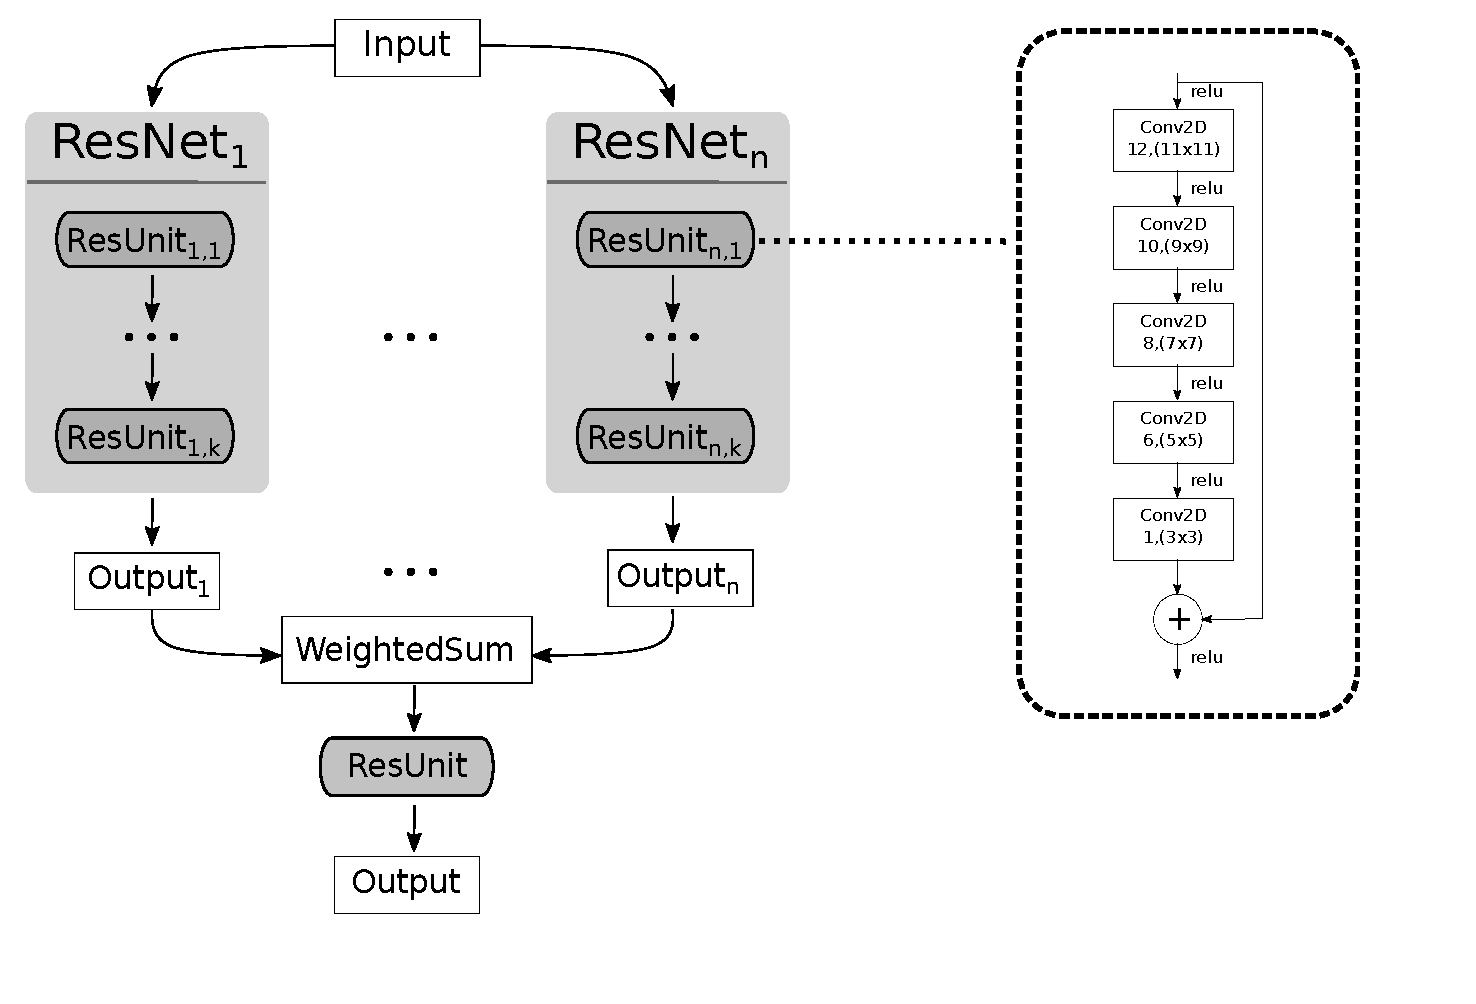
\includegraphics[width=10cm]{pics/nn.pdf}
\caption{Parallel residual neural network architecture}
\label{nn}
\end{center}
\end{figure} 

\subsection{Experiments}


%
\bibliography{main} 
\bibliographystyle{ieeetr}
\end{document}
